\documentclass{article}
\usepackage{amsmath}
\usepackage{amssymb}
\usepackage{graphicx}
\usepackage{hyperref}
\usepackage[version=4]{mhchem}


\begin{document}
\section*{Problem}
\(P A\) and \(P B\) are tangent to circle \(O\) at \(A\) and \(B\), respectively. \(A C\) is the diameter of circle \(O\). Prove: \(B C / / P O\).\\
\centering
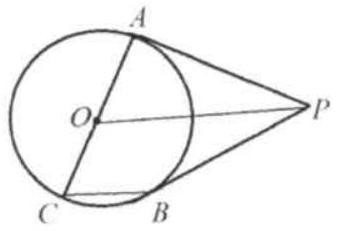
\includegraphics[width=\textwidth]{images/169(4).jpg}

\section*{Solution}
Method 1:\\
Connect \(A B\). Extend \(P B\) to \(E\).\\
Since \(P A\) and \(P B\) are tangent to circle \(O, \angle A P D=\angle B P D\) \(=\alpha, \angle P A O=90^{\circ}, \angle P D A=90^{\circ}\),\\
Let \(\angle P O A=\beta\).\\
\(\angle D A O+\angle D O A=\angle D A O+\beta=90^{\circ}\).\\
\(\angle A P O+\angle D O A=\alpha+\beta=90^{\circ}\).\\
So \(\angle D A O=\alpha\).\\
\centering
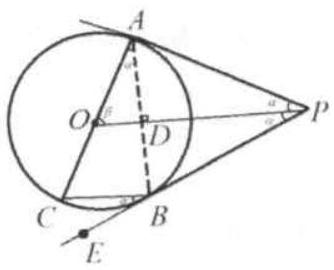
\includegraphics[width=\textwidth]{images/171(1).jpg}\\
\(\angle C A B=\angle C B E\) (both face the same \(\operatorname{arc} B C\) ).\\
So \(\angle C B E=\alpha\).\\
Thus \(B C / / P O\).

Method 2:\\
Connect \(A B\).\\
Since \(P A\) and \(P B\) are tangent to circle \(O, \angle A D P=\) \(\angle B D P=90^{\circ}, P D \perp A B\) or \(P O \perp A B\)\\
Since \(A C\) is the diameter,\\
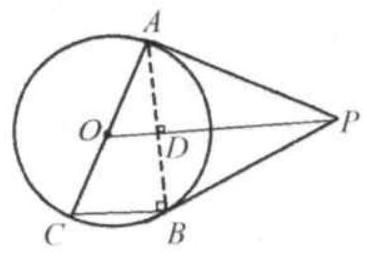
\includegraphics[width=\textwidth]{images/171(2).jpg} \(\angle A B C=90^{\circ} . B C \perp A B\).\\
Thus \(B C / / P O\).

\end{document}
